\section{The Perturbation Profile}
\subsection{Setting}
A trial is a time-ordered sequence of fixations $\{(x_k, y_k, d_k)\}_{k=1}^{n}$ with locations in a common frame and durations $d_k$. A descriptor $f$ maps a trial to a feature vector. A task supplies a binary label and a participant identifier per trial. Performance is the AUC of out-of-fold decision values from participant-held-out cross-validation: participants are split into ten folds and all trials of a participant are held out together, so no participant contributes to both training and test, and features are standardized on the training folds only. A cross-validated AUC can be computed in two ways. The \emph{pooled} AUC ranks all out-of-fold decision values together. Pooling compares scores produced by different fitted models, and differences in their score offsets and in the class proportions of their training folds can bias it; with little or no signal, the bias is usually downward \citep{parker2007stratification, airola2011comparison}, most of all when the label is constant within participants and the folds differ in their class mix. A perturbation can change this bias as well as the discrimination, so a difference between observed and transformed pooled AUCs can contain both. The primary analysis therefore uses the \emph{within-fold} AUC, the AUC over positive--negative pairs drawn from the same test fold (equivalently, the per-fold AUCs averaged with weights proportional to their numbers of pairs), with \emph{class-balanced} folds: participants are dealt to the folds within each class, so that every fold receives a similar mix of classes. Within a fold all scores come from one model, so offsets between models cannot enter. Every profile is repeated with the pooled AUC as a sensitivity analysis. Cross-validation estimates the performance of the fitting procedure over training sets rather than that of one fitted model \citep{bates2024cross}, which is the quantity a pipeline-level sensitivity requires. A within-participant AUC would remove participant offsets too, but it answers a different question and is undefined for the five problems whose label is constant within participants. The learner is a linear support vector machine (liblinear, $C = 1$) on standardized features; the framework accepts any scikit-learn estimator.

\subsection{Transformations}\label{sec:transf}
Each transformation $\tau$ is applied independently to every trial (Table~\ref{tab:nulls}; Figure~\ref{fig:schematic}). Each targets a stated property while preserving an explicitly listed set of invariants, and interpretation depends on that list: a sensitivity to $\tau$ is a sensitivity to whatever $\tau$ changes, which is always the named property together with anything that depends on it.

\begin{table}[!htbp]
\centering\small
\caption{The five transformations, with what each destroys and what each preserves. For the first four the preservation statements are exact; jitter is a gradual perturbation, and its row describes distribution-level effects. The last column names the property a transformation does \emph{not} remove although its name might suggest it.}
\label{tab:nulls}
\begin{adjustwidth}{-\extralength}{0cm}
\centering
\begin{tabular}{p{2.1cm}p{3.4cm}p{2.5cm}p{3.5cm}p{2.5cm}}
\toprule
Transf. & Operation & Destroys & Preserves & Not removed \\
\midrule
order & permute the fixation sequence & serial order & multisets of locations and durations; every order-free property & --- \\
duration coupling & permute durations across the trial's fixations & which fixation carries which duration, and with it any dependence of duration on sequence position (trends, serial autocorrelation) & locations, order, the trial's duration distribution (mean, spread, total dwell, count) & marginal duration information \\
duration marginal & redraw the trial's durations from the pooled durations of the other participants & the trial's duration distribution, the coupling and the duration--sequence dependence & locations, order, count & --- \\
rotation & rigid rotation (uniform angle) and random reflection about a centre & orientation, side relative to the stimulus, and handedness (chirality) & all pairwise distances and unsigned angles, order, durations, each fixation's eccentricity from the centre & eccentricity; any rotationally invariant location contrast (exact) \\
jitter($s$) & add isotropic Gaussian noise, SD $s$, to every location & fine spatial structure, increasingly with $s$ (shorthand; not a band-pass filter) & order and durations (exact); orientation and structure coarser than $s$ approximately, at the distribution level & --- \\
\bottomrule
\end{tabular}
\end{adjustwidth}
\end{table}

The \emph{order} transformation removes only the sequence. It can also change what an order-dependent feature measures, and for one common feature the change is exact. Let a trial have fixations at $p_1,\dots,p_n$ ($n \geq 2$), let $A = (n-1)^{-1}\sum_{k=1}^{n-1}\lVert p_{k+1} - p_k\rVert$ be its mean saccade amplitude, and let $\bar D = [n(n-1)]^{-1}\sum_{i \neq j}\lVert p_i - p_j\rVert$ be its mean pairwise distance. \emph{Proposition.} If $\pi$ is a uniformly random permutation of $\{1,\dots,n\}$ and $A_\pi$ the mean amplitude of the permuted sequence, then $\mathbb{E}_\pi[A_\pi] = \bar D$. \emph{Proof.} For each $k$, the pair $(\pi(k), \pi(k+1))$ is uniformly distributed over the $n(n-1)$ ordered pairs of distinct indices, so $\mathbb{E}_\pi\lVert p_{\pi(k+1)} - p_{\pi(k)}\rVert = \bar D$; averaging over $k$ gives the result. $\square$ After order permutation, mean saccade amplitude is therefore an unbiased, noisy measurement of spatial spread; it carries no sequential information. Section~\ref{sec:against} uses this result. The \emph{duration-coupling} transformation removes the assignment of durations to fixations. That assignment includes more than it may seem: any trend of duration along the trial and any serial dependence between successive durations are destroyed too, so a sensitivity to this transformation cannot say which of these carried the signal (the duration-trend simulation of Section~\ref{sec:sim} is a case in point). Because it preserves the trial's duration distribution, a descriptor that reads mean or total duration is invariant to it, and a task in which one class simply fixates longer would show zero sensitivity to it. The \emph{duration-marginal} transformation replaces the trial's durations by a draw without replacement from a donor pool, which destroys the trial's own distribution (and, with it, the coupling). The pool holds every fixation duration of the problem's \emph{other} participants, so no trial receives durations of its own participant. The pool is built once on the full dataset and is not rebuilt inside cross-validation or bootstrap draws, so held-out participants donate durations to trials in the training folds; the transformation is transductive in that limited sense. Rebuilding the pool from the training participants of each fold changed the classic descriptor's duration-marginal sensitivity by at most 0.007 AUC on the three problems where that sensitivity is interpreted, and by at most 0.064 on any problem, the largest changes falling on problems without signal whose intervals are wider than 0.3 (Table S24 in Online Resource 1). The \emph{rotation} transformation is a rigid motion about a centre: every intra-scanpath distance and every temporal relation is preserved, and so is every fixation's distance from the centre; it destroys orientation and side. Because half of the draws also reflect the scanpath, it destroys handedness as well: clockwise and counter-clockwise circulation, or left-to-right and right-to-left sweeps, are exchanged. We include the reflection so that a descriptor reading handedness cannot pass the transformation unchanged; the cost is that a rotation sensitivity alone does not separate orientation from handedness. The package therefore also offers the rotation without reflection. A class contrast between central and peripheral viewing survives either version entirely, which we demonstrate in Section~\ref{sec:sim}; the transformation is therefore a test of rotation/reflection sensitivity, not of stimulus location in general. For a descriptor whose spatial support is bounded (a triangulation of a stimulus's areas of interest), rotation about the frame centre can sweep fixations off the support and register as a spurious sensitivity, so we rotate such descriptors about the support's centre. That reduces the problem but does not remove it: a rectangle or an irregular set of anchors does not map onto itself under rotation, and jitter moves fixations near the boundary out of it as well. A fixation that falls outside the triangulation lies in no triangle and is dropped from the graph. We therefore report the share of fixations and dwell time each transformation leaves on the support, by class, and check the interpreted sensitivities with support-matched transformations (Section~\ref{sec:support}). The \emph{jitter} transformation perturbs each location by $\mathcal{N}(0, s^2 I)$; two originally coincident fixations end up on average $s\sqrt{\pi}$ apart (root-mean-square $2s$). Jitter preserves order and durations exactly and nothing else exactly: it is a gradual perturbation that changes pairwise distances, amplitudes, local density, orientation and region membership together, more at fine scales than at coarse ones. ``Spatial structure finer than $s$'' is therefore operational shorthand for what the transformation mostly disturbs, not a filter with a cut-off. Sweeping $s$ produces a curve of AUC against scale from which we report two summaries with explicit definitions (Section~\ref{sec:stat}).

\begin{figure}[!htbp]
\centering
\begin{adjustwidth}{-\extralength}{0cm}
\centering
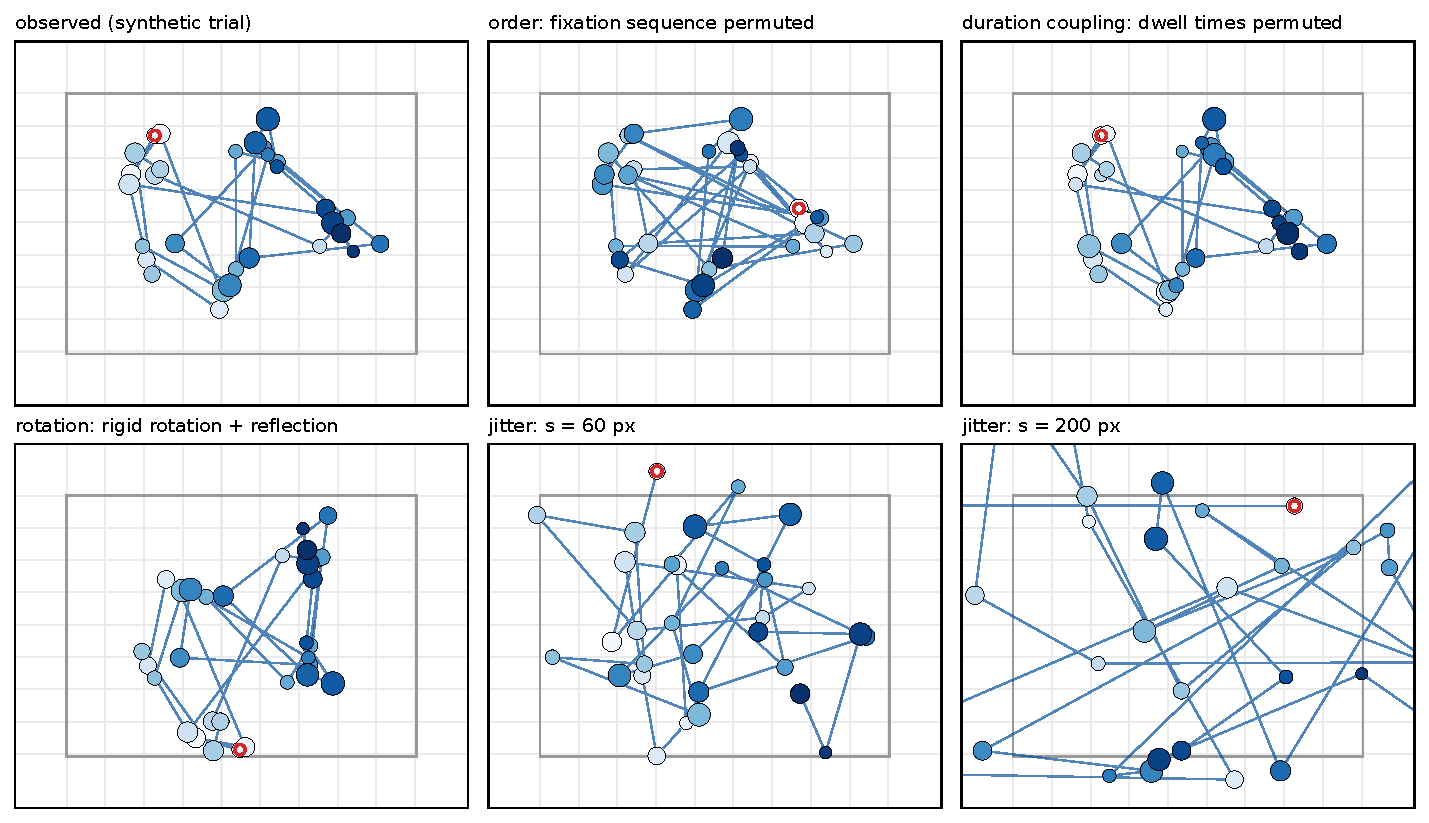
\includegraphics[width=\linewidth]{fig_nulls_schematic}
\end{adjustwidth}
\caption{One \emph{synthetic} trial in the analysis window under each transformation; no participant's gaze is shown. Marker size is fixation duration, colour is order (light to dark), the red ring is the first fixation, the light grid is the tiling of the directed graph (Section~\ref{sec:desc}). Shown are four of the five transformations (duration marginal would look like duration coupling with different marker sizes). Order permutation keeps the points and re-threads the path; duration coupling keeps the path and re-sizes the markers; rotation keeps every distance, angle and eccentricity and changes orientation and side; jitter at 60 px perturbs fine spatial structure, at 200 px coarse structure.}
\label{fig:schematic}
\end{figure}

\subsection{Sensitivity, and What It Is Not}\label{sec:stat}
For a transformation $\tau$ we draw $R$ independent replicates, recompute features and participant-held-out decision values on each, and set $\AUC_\tau = R^{-1}\sum_r \AUC(\tau_r)$. The \emph{sensitivity} of the descriptor to $\tau$ is $\Cs_\tau = \AUC_{\mathrm{obs}} - \AUC_\tau$. A negative sensitivity means that the transformed pipeline discriminates better than the observed one. It has two possible sources, and they must be told apart. The transformation can make information accessible that the observed features express poorly (the Proposition of Section~\ref{sec:transf} gives an exact case), or it can change the evaluation's bias, for example by moving an AUC that lies below its null distribution back towards that null. We separate them with three permutation distributions, built with the problem's own permutation scheme (Section~\ref{sec:inf}) on the same transformed trials: for the observed AUC, for the transformed AUC, and for the contrast $\Cs_\tau$ itself. A negative sensitivity is read as information made accessible when the transformed AUC exceeds its null and $\Cs_\tau$ lies below the null distribution of the contrast. It is read as a change in evaluation bias when the observed AUC lies below its null and the transformed AUC does not exceed its own. A significant observed AUC is therefore not required for a negative sensitivity to be informative.

The classifier is refit on the transformed trials, so $\Cs_\tau$ is the discrimination a \emph{pipeline} (descriptor plus learner plus evaluation) loses when the property is destroyed and it is allowed to adapt. It is not a measurement of what the originally fitted classifier relied on. A refitted learner can move to information that is redundant with the destroyed property, so a sensitivity of zero is consistent with the original model having leaned on that property heavily; only the pipeline's \emph{achievable} discrimination is shown to be unaffected. We use \emph{sensitivity} throughout in that pipeline sense.

Refitting follows established practice. \citet{hooker2019benchmark} retrain on the modified data because re-scoring the original model confounds the information removed with the artefact of moving off the training distribution, and \citet{hooker2021unrestricted} show that permuting a feature that depends on others forces that extrapolation. A perturbation profile applies the same remedy to whole trials, with one advantage: each transformation preserves stated invariants, so a transformed trial is still a scanpath, with the same number of fixations and, under three of the five transformations, the same set of locations. What the refit costs is the pipeline reading above.

Three caveats govern interpretation. First, $\Cs_\tau$ is a property of the descriptor, learner, evaluation, task, and transformation jointly; it is not a share of information in the behaviour, and $\sum_\tau \Cs_\tau$ need not equal the distance of $\AUC_{\mathrm{obs}}$ from its permutation null. Second, zero sensitivity is ambiguous between invariance of the descriptor, redundancy of the property with others the descriptor also reads (which refitting is free to exploit), insufficient precision, and information the transformation leaves intact. Third, the transformations are applied separately, not sequentially, so the profile does not partition the signal; interactions and redundancy are visible only by comparing descriptors that read different properties, which is how we use the baselines below.

For the jitter sweep, two summaries are used in the simulations of Section~\ref{sec:sim}, where the planted scale is known; for the real data we report the sweep itself. The \emph{first-exclusion scale} is the first tested grid point at which the pointwise 95\% interval for $\Cs$ excludes zero. It is a pointwise, unadjusted quantity: the intervals along the sweep are neither simultaneous nor corrected for the number of grid points, so it is not an estimate of where sensitivity begins, and it moves with the grid, the sample size and the Monte-Carlo settings. The \emph{half-loss bracket} is the pair of adjacent tested scales between which the point estimate $\Cs$ first exceeds half of $\AUC_{\mathrm{obs}} - \AUC_0$, where $\AUC_0$ is the mean of the observed AUC's permutation distribution (0.5 is not used as the reference, because the null is not centred there); it uses no interval. Neither locates a spatial scale of the behaviour. The primary result of a sweep is the curve of sensitivities with their intervals (Figure~\ref{fig:profiles}; Tables S1--S13 in Online Resource 1); the two summaries are reading aids for it.

\subsection{Inference}\label{sec:inf}
Trials are clustered within participants, and cross-validated AUCs have no unbiased variance estimator because folds share training data \citep{varoquaux2018cross}. Resampling participants over the \emph{fixed} out-of-fold scores (the fixed-score bootstrap) captures trial-sampling variance but not the variance of refitting the classifier, so its intervals are too narrow wherever refitting varies. We therefore use a \emph{refit bootstrap}: participants are resampled with replacement (duplicates keep their identity, so folds remain participant-pure), the classifier is refit by participant-held-out cross-validation on the resampled observed features and on one randomly chosen transformed replicate, and the two AUCs $a_{\mathrm{obs}}$ and $a_{\tau}$ are recorded over $B$ draws.

The estimator averages the transformed AUC over $R$ replicates, whereas each bootstrap draw uses one, so the bootstrap variance of $a_{\mathrm{obs}} - a_\tau$ overstates the estimator's variance. Write $a_\tau^{(b)} = g(\text{sample}_b) + e_b$, where $g$ is the participant-sampling component and $e_b$ the Monte-Carlo component of drawing one replicate, assumed independent of the participant resample with variance $v_e$ not depending on the resample. Then $\mathrm{Var}_b(a_\tau) = v_g + v_e$, whereas the estimator's transformed term has variance $v_g + v_e/R$, giving
\begin{equation}
\widehat{\mathrm{Var}}(\Cs_\tau) = \mathrm{Var}_b(a_{\mathrm{obs}}) + \big[\mathrm{Var}_b(a_{\tau}) - \hat v_e\big] + \hat v_e/R - 2\,\mathrm{Cov}_b(a_{\mathrm{obs}}, a_{\tau}),
\label{eq:var}
\end{equation}
where $\hat v_e$ is the sample variance of the $R$ replicate AUCs on the full data, capped at $\mathrm{Var}_b(a_\tau)$, and a normal-approximation 95\% interval is placed around $\Cs_\tau$. Two cases are handled separately. A cell is reported as ``0 (exact)'' with no interval when the transformation leaves the \emph{feature matrix} unchanged: when $f(\tau_r(\text{trial})) = f(\text{trial})$ to within $10^{-9}$ for every trial in every one of the $R$ replicates. The sensitivity is then identically zero under every resample and its sampling variance is zero. Every ``0 (exact)'' cell below is an invariance that holds analytically for the descriptor (recurrence reads only pairwise distances; the dispersion and count baselines read no order), verified by feature equality on the replicates drawn. A \emph{degenerate} cell, in which every bootstrap draw gives $a_{\mathrm{obs}} = a_\tau$ without the features being equal (which occurs at ceiling), is marked separately. If the corrected variance is not positive for a non-invariant cell, the uncorrected paired bootstrap variance $\mathrm{Var}_b(a_{\mathrm{obs}} - a_\tau)$ is used instead, which under the assumptions of Equation~\ref{eq:var} has expectation larger by $v_e(1 - 1/R)$; a larger variance estimate is not by itself a coverage guarantee, since it addresses neither bias nor the normal approximation, and the cell is flagged. Writing Equation~\ref{eq:var} under the constant-$v_e$ assumption does not verify it. Section~\ref{sec:sim} checks the coverage of the resulting interval by simulation and compares it with a \emph{direct} refit bootstrap that averages all $R$ transformed replicates inside every draw, which needs no correction but costs $R$ times as much.

The interval is built around $\Cs_\tau$ for the dataset in hand; what a simulation can check coverage against is
\begin{equation}
\theta_\tau = \mathbb{E}_D\big[\AUC_{\mathrm{obs}}(D) - \mathbb{E}_r \AUC_{\tau,r}(D)\big],
\label{eq:estimand}
\end{equation}
the expectation, over datasets $D$ from a generative design, of the finite-sample participant-held-out contrast. This is a \emph{procedural} estimand: it is defined by the design together with the participant count, the descriptor, the learner and the participant-held-out evaluation, so a study with more participants defines a different $\theta_\tau$ and the value estimated here transfers to no other sample size. Section~\ref{sec:sim} estimates $\theta_\tau$ on datasets whose seeds are disjoint from those whose intervals are assessed. Averaging replicate AUCs, rather than averaging decision values across replicates before computing an AUC, also matters: the latter ensembles the replicates into a different classifier, which can change $\AUC_\tau$ and, when it raises it, biases $\Cs_\tau$ downward.

All intervals below are unadjusted 95\% intervals and are exploratory: each profile comprises eight columns (five transformations, jitter at four scales), and the families across descriptors and problems are large. The estimates and their intervals are the primary result. The markers in the tables (an interval excluding zero; an interval inside the margin) are reading aids that dichotomize them, and we do not treat an isolated exclusion as a confirmed finding or an interval that covers zero as evidence of absence. For the latter we use an explicit equivalence margin: a sensitivity is called \emph{negligible} only when its whole interval lies within $\pm 0.05$ AUC; otherwise it is \emph{inconclusive}. An interval can both exclude zero and lie within the margin, in which case the effect is \emph{nonzero but negligible}. The margin is a judgement of practical relevance. We set it at $0.05$ AUC as the tolerance we would apply in this application (a shift of less than five hundredths of an AUC point is not, in our judgement, a reason to describe a descriptor as reading a property), and a reader with a different tolerance should reclassify accordingly. It is not justified by ranking preservation. The behaviour of the call near the margin was not re-examined by simulation for this pipeline, so we use it only as a reading aid. The margin is applied only to genuine intervals, never to exact invariances.

\paragraph{Permutation tests.} Each observed AUC is compared with a permutation distribution \citep{ojala2010permutation} of 1000 permutations ($p = (1 + \#\{\text{permuted AUC} \geq \text{observed}\})/1001$); its mean and SD and the lower-tail probability are stored with it. Labels are permuted at the level at which they were assigned and within blocks that keep the design's structure: whole participants for a label that is constant within participants, passages within participants for SB-SAT comprehension (the pages of a passage share its outcome), the two halves within each recording for the half problems, answers within each program for pooled correctness (so that the association of correctness with the program is preserved under the null), and trials within participants otherwise (Table~\ref{tab:perm}). The same schemes give the nulls of transformed AUCs and of contrasts.

\paragraph{Which sensitivities are interpreted.} A profile of eight columns for each of ten descriptor variants on thirteen problems produces several hundred intervals, and reading off those that exclude zero would capitalize on chance. We therefore fix a rule. A cell is \emph{interpreted} only if the observed AUC exceeds its permutation distribution ($p \leq 0.05$), the refit-bootstrap interval of the observed AUC lies above 0.5, and the sensitivity interval excludes zero. An interpreted cell is \emph{robust} if its sign and the exclusion of zero hold as well with the pooled AUC, in every one of 20 fold partitions (for the sign of the point estimate), in three longer runs ($R = 20$, $B = 300$) and, for a descriptor with bounded support, on a version of the descriptor that loses no fixation under any transformation. The result under a second learner is reported alongside. A negative sensitivity on a problem whose observed AUC does not exceed its null can still be informative by the three-null argument of Section~\ref{sec:stat}, but it is outside the rule and we report such cases without building on them.

\begin{table}[!htbp]
\centering\small
\caption{Permutation schemes. For each problem: the unit at which the label was assigned, the unit whose labels are permuted, the block within which they are permuted, and what every permutation preserves.}
\label{tab:perm}
\resizebox{\linewidth}{!}{\begin{tabular}{>{\raggedright\arraybackslash}p{3.3cm}>{\raggedright\arraybackslash}p{2.6cm}>{\raggedright\arraybackslash}p{2.6cm}>{\raggedright\arraybackslash}p{2.4cm}>{\raggedright\arraybackslash}p{4.1cm}}
\toprule
Problems & Label assigned to & Unit permuted & Block & Preserved under the null \\
\midrule
\texttt{gb\_tex\_vd1}, \texttt{gb\_vd1\_blg}, \texttt{gb\_vd1\_vd2}, \texttt{gb\_tex\_s1s2}, \texttt{em\_program} & trial (task, stimulus or session) & trial & participant & each participant's label counts; participant clustering \\
\texttt{gb\_vd1\_halves}, \texttt{em\_halves} & half of one recording & half & recording (participant $\times$ session or program) & one first and one second half per recording \\
\texttt{sb\_native}, \texttt{em\_expertise}, \texttt{em\_correctrect}, \texttt{em\_correctveh} & participant & participant (all trials together) & all participants & the number of participants per class; all trials of a participant share one label \\
\texttt{sb\_compr} & passage (its pages share one outcome) & passage & participant & each participant's passage-label counts; pages of a passage share one label \\
\texttt{em\_correct} & answer to one program & trial & program & the number of correct and incorrect answers within each program \\
\bottomrule
\end{tabular}
}
\end{table}

\subsection{Invariance Checks}
Some (descriptor, transformation) pairs must return $\Cs = 0$ exactly: order for any order-free descriptor; duration coupling and duration marginal for any descriptor that does not read durations; rotation for any descriptor that depends only on pairwise distances or on the distance matrix. These serve as checks that the machinery is correct, not as evidence about the data. They held in every analysis below.

